\documentclass[12pt]{article}
\usepackage[english]{babel}
\usepackage{natbib}
\usepackage{url}
\usepackage[utf8x]{inputenc}
\usepackage{amsmath}
\usepackage{graphicx}
\graphicspath{{../docs/img/}}
\usepackage{parskip}
\usepackage{fancyhdr}
\usepackage{vmargin}
\usepackage{xcolor}
\usepackage{booktabs}
\usepackage{float}
\usepackage{pgfplots}
\usepackage{tikz}
\pgfplotsset{width=10cm,compat=1.9}

\setmarginsrb{3 cm}{2.5 cm}{3 cm}{2.5 cm}{1 cm}{1.5 cm}{1 cm}{1.5 cm}

\title{Sprint 1 Backlog}								% Title
\author{Thierry's Minions}								% Author
\date{12 Sept 2015}											% Date

\makeatletter
\let\thetitle\@title
\let\theauthor\@author
\let\thedate\@date
\makeatother

\pagestyle{fancy}
\fancyhf{}
\rhead{\theauthor}
\lhead{\thetitle}
\cfoot{\thepage}

\newcommand*{\userstory}[5][.25em]{
%  \begin{tabular*}{\maincolumnwidth}{l@{\extracolsep{\fill}}r}%
%    {\bfseries #2} & {\bfseries #4}\\%
%    {#3}\\%
%  \end{tabular*}%
%  \ifx&#5&%
%  \else{\\%
%    \begin{minipage}{\maincolumnwidth}%
%      #5%
%    \end{minipage}}\fi%
%  \par\addvspace{#1}
\textbf{#1} 
  }

\newcommand{\roundpic}[4][]{
  \tikz\node [circle, minimum width = #2,
    path picture = {
      \node [#1] at (path picture bounding box.center) {
        \includegraphics[width=#3]{#4}};
    }] {};}

\begin{document}

%%%%%%%%%%%%%%%%%%%%%%%%%%%%%%%%%%%%%%%%%%%%%%%%%%%%%%%%%%%%%%%%%%%%%%%%%%%%%%%%%%%%%%%%%

\begin{titlepage}
	\centering
    \vspace*{0.5 cm}
\roundpic[]{9cm}{9cm}{leader.jpg}

    \textsc{\LARGE Thierry's Minions/Team25\\[0.5em] Deliverable 3}\\[2.0 cm]	
	\textsc{\Large CSCC01 Fall 2018}\\[0.5 cm]				% Course Code
	\rule{\linewidth}{0.2 mm} \\[0.4 cm]
	{ \huge \bfseries \thetitle}\\
	\rule{\linewidth}{0.2 mm} \\[1.5 cm]
	
	\begin{minipage}{0.4\textwidth}
		\begin{flushleft} \large
			\emph{Submitted To:}\\
			Saba Kiaei\\
            Teaching Assistant\\
            Computer Science Department\\
			\end{flushleft}
			\end{minipage}~
			\begin{minipage}{0.4\textwidth}
            
			\begin{flushright} \large
			\emph{Submitted By :} \\
			Rishabh Kaant Sharma\\
            Joseph Sokolon\\
            Balaji Badu\\
            Jayden Arquelada\\
            Edgar Sarkisian\\
		\end{flushright}
        
	\end{minipage}\\[2 cm]
	
	
    
    
    
    
	
\end{titlepage}

%%%%%%%%%%%%%%%%%%%%%%%%%%%%%%%%%%%%%%%%%%%%%%%%%%%%%%%%%%%%%%%%%%%%%%%%%%%%%%%%%%%%%%%%%

\textcolor{black}{\tableofcontents}
\pagebreak

%%%%%%%%%%%%%%%%%%%%%%%%%%%%%%%%%%%%%%%%%%%%%%%%%%%%%%%%%%%%%%%%%%%%%%%%%%%%%%%%%%%%%%%%%

\section{Sprint Tasks}

\subsection{Task 1A: Setup server}
\begin{itemize}%
\item Story Points: 5
\item Setup server using nodejs.
\item Don't need to setup persistent database, create mock database using javascript.
\item Database will be called database.js
\item Create login endpoint
\item Login endpoint will be a http POST request to: /login/org-user/
\item Body of request will have json with login information: 
\item \{username: John, password: pass1\}
\end{itemize}

\subsection{Task 1B: Setup database}
\begin{itemize}%
\item Story Points: 2
\item This task has a dependency on task 1A
\item Setup persistent SQL database using Amazon Web Services.
\item Connect server to database
\item Replace functions implementations in database.js to use the real database
\end{itemize}

\subsection{Task 1C: Create Login Page}
\begin{itemize}%
\item Story Points: 8
\item Create Login page for the Desktop Application
\item Desktop Application will be written in Java and use JavaFX for UI Library
\item Application must be simple to compile and run
\item Login page will have 2 fields, username and password
\item Login page will have a login button
\end{itemize}

\subsection{Task 1D: Create Login Controller}
\begin{itemize}%
\item Story Points: 3
\item This task has a dependency on task 1A
\item Create Login Controller Class for the Desktop Application
\item Controller should contain implementation for sending login information to server
\item Controller should recieve response from server and distinguish between successful and unsuccessful login  
\end{itemize}

\subsection{Task 1E: Integrate Login UI and Controller}
\begin{itemize}%
\item Story Points: 2
\item This task has a dependency on task 1C, 1D
\item Integrate the login controller with the UI
\item The login request should be sent when button is clicked on UI
\item The UI should reflect whether the login operation was successful
\end{itemize}

\subsection{Task 1F: Test entire flow}
\begin{itemize}%
\item Story Points: 1
\item This task has a dependency on all previous task in story 
\item Test the entire workflow of login (Client + Server)
\item Fix any errors 
\end{itemize}

\newpage
\section{Sprint Plan}
\textbf{Sprint 1 : October 6th - October 12th (Saturday - Friday)}
\begin{table}[H]
\begin{tabular}{@{}c|c|c|c|ccccccc@{}}
\toprule
Story & Task & Dependency & \begin{tabular}[c]{@{}c@{}}Story\\ Points\end{tabular} & \begin{tabular}[c]{@{}c@{}}Day\\ 1\end{tabular} & \begin{tabular}[c]{@{}c@{}}Day\\ 2\end{tabular} & \begin{tabular}[c]{@{}c@{}}Day \\ 3\end{tabular} & \begin{tabular}[c]{@{}c@{}}Day \\ 4\end{tabular} & \begin{tabular}[c]{@{}c@{}}Day \\ 5\end{tabular} & \begin{tabular}[c]{@{}c@{}}Day \\ 6\end{tabular} & \begin{tabular}[c]{@{}c@{}}Day \\ 7\end{tabular} \\ \midrule
1     & A    &            & 5                                                      & RS:2                                            & RS:3                                            &                                                  &                                                  &                                                  &                                                  &                                                  \\
1     & B    & A          & 2                                                      &                                                 &                                                 & JS:2                                             &                                                  &                                                  &                                                  &                                                  \\
1     & C    &            & 8                                                      & ES:2                                            & ES:2                                            & ES:4                                             &                                                  &                                                  &                                                  &                                                  \\
1     & D    & A          & 3                                                      &                                                 &                                                 & JA:3                                             &                                                  &                                                  &                                                  &                                                  \\
1     & E    & C, D       & 2                                                      &                                                 &                                                 &                                                  & BB:2                                             &                                                  &                                                  &                                                  \\
1     & F    & ALL        & 1                                                      &                                                 &                                                 &                                                  &                                                  & JS:1                                             &                                                  &                                                  \\ \bottomrule
\end{tabular}
\end{table}

\begin{itemize}%
\item Estimated story points team can complete: 21
\item Rishabh will complete task 1A by end of day 2.
\item Joey will complete task 1B by end of day 3.
\item Edgar will complete task 1C by end of day 3.
\item Jayden will complete task 1D by end of day 3.
\item Balaji will complete task 1E by end of day 4.
\item Joey will complete task 1F, and release feature by end of day 5.
\item The team believes they can complete User Story 1 by end of the day 5. 
\end{itemize}

\newpage

\section{Sprint Report}
\textbf{Sprint 1 : October 6th - October 12th (Saturday - Friday)}

\begin{table}[H]

\begin{tabular}{@{}l|c|c|c|ccccccc@{}}
\toprule
Story & Task & Dependency & \begin{tabular}[c]{@{}c@{}}Story\\ Points\end{tabular} & \begin{tabular}[c]{@{}c@{}}Day\\ 1\end{tabular} & \begin{tabular}[c]{@{}c@{}}Day\\ 2\end{tabular} & \begin{tabular}[c]{@{}c@{}}Day\\ 3\end{tabular} & \begin{tabular}[c]{@{}c@{}}Day\\ 4\end{tabular} & \begin{tabular}[c]{@{}c@{}}Day\\ 5\end{tabular} & \begin{tabular}[c]{@{}c@{}}Day\\ 6\end{tabular} & \begin{tabular}[c]{@{}c@{}}Day\\ 7\end{tabular} \\ \midrule
1     & A    &            & 5                                                      &                                                 &                                                 &                                                 & RS:3                                            & RS:5                                            &                                                 &                                                 \\
1     & B    & A          & 2                                                      &                                                 &                                                 &                                                 &                                                 & JS:3                                            &                                                 &                                                 \\
1     & C    &            & 8                                                      &                                                 & ES:8                                            & ES:4                                            &                                                 &                                                 &                                                 &                                                 \\
1     & D    & A          & 3                                                      &                                                 &                                                 &                                                 & JA:3                                            &                                                 &                                                 &                                                 \\
1     & E    & C, D       & 2                                                      &                                                 &                                                 &                                                 &                                                 &                                                 &                                                 &                                                 \\
1     & F    & ALL        & 1                                                      &                                                 &                                                 &                                                 &                                                 &                                                 &                                                 &                                                 \\ \bottomrule
\end{tabular}
\end{table}

\begin{itemize}%
\item Actual story points burned: 18
\item Edgar didn't start task 1C until day 2.  It took Edgar 4 hours longer then expected. 
\item Rishabh didn't start task 1A until day 4, and finished on day 5. It took Rishabh 3 hours longer then expected. 
\item Joey finished task 1B on the same day task 1A was completed.
\item Jayden started task 1D a day late. He completed the task on the same day.
\item Balaiji wasn't able to work on task 1E for the sprint due to other school commitments.
\item The team didn't complete user story 1 by end of the sprint 1.Remaining tasks will be carried over to sprint 2. 
\end{itemize}

\section{Sprint Burndown Chart}

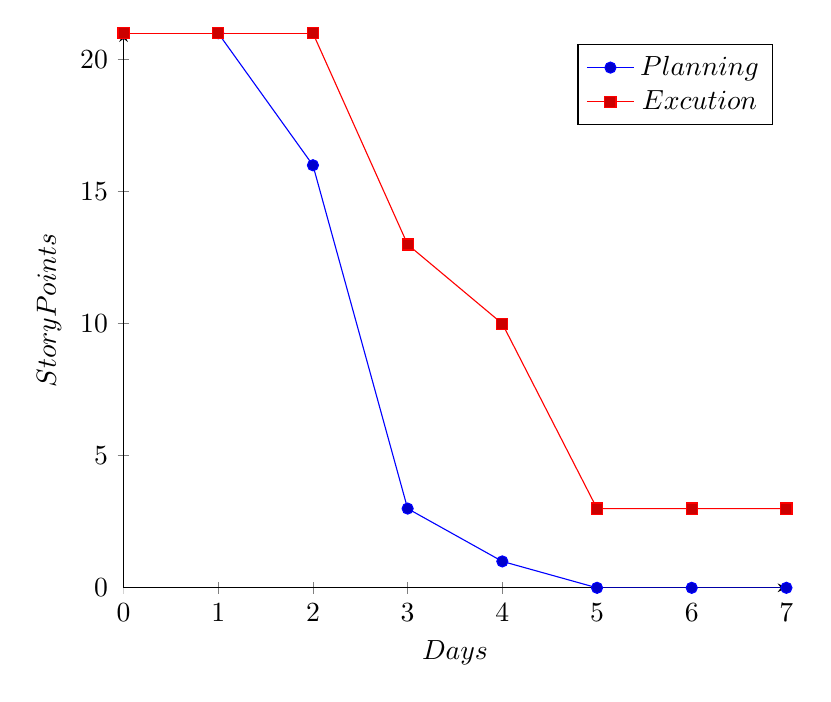
\begin{tikzpicture}
\begin{axis}[
    axis lines = left,
    xlabel = $Days$,
    ylabel = {$Story Points$},
]
\addplot coordinates {(0,21) (1,21) (2,16) (3,3) (4,1) (5,0) (6,0) (7,0)};
\addlegendentry{$Planning$}
\addplot coordinates {(0,21) (1,21) (2,21) (3,13) (4,10) (5,3) (6,3) (7,3)};
\addlegendentry{$Excution$}
\end{axis}
\end{tikzpicture}

\newpage
\bibliographystyle{plain}
\bibliography{biblist}

\end{document}